% Chapter 4
\chapter{تعویض مدل‌های شبکه عصبی بین کاربران}

\section{مقدمه}
در فصل پیشین، روش‌های متعددی برای حل مشکل داده‌های
\lr{non-IID}
مورد بررسی قرار گرفتند. در این فصل، رویکرد جامعی برای مقابله با این چالش، یعنی تبادل مدل‌های شبکه عصبی میان کاربران نهایی، بررسی می‌شود که محور اصلی این پایان‌نامه را تشکیل می‌دهد. به منظور درک بهتر، ابتدا یک مثال از داده‌های
\lr{non-IID}
مطرح خواهد شد.

فرض کنید هدف، آموزش مدلی برای تشخیص اشیا مانند علائم ترافیکی و علائم فروشگاهی است. اگر وسایل نقلیه به ترتیب در بزرگراه و مرکز شهر حرکت کنند، داده‌های ویدیویی آن‌ها توزیع‌های متفاوتی از این علائم خواهند داشت. به این معنا که داده‌های آموزشی جمع‌آوری شده از بزرگراه ممکن است کمتر شامل علائم فروشگاهی باشند، در حالی که داده‌های جمع‌آوری شده از مرکز شهر حاوی تعداد بیشتری از هر دو نوع علائم خواهند بود. این تفاوت در توزیع داده‌ها در دستگاه‌های نهایی می‌تواند باعث ایجاد مشکل انحراف وزن‌ها شود.

برای حل این مسئله، عملیات تعویض مدل‌های شبکه عصبی بین کاربران نهایی پیشنهاد می‌شود. این رویکرد، مدل‌ها را بین دستگاه‌های نهایی جابجا می‌کند تا تنوع داده‌ها در دستگاه‌های مختلف کاهش یابد. این عملیات بدون نیاز به هزینه‌های محاسباتی و ارتباطی اضافی، به بهبود عملکرد مدل در مواجهه با داده‌های
\lr{non-IID}
کمک می‌کند.

در این فصل ابتدا ...

\section{
	روش تعویض فدرال%
\LTRfootnote{Federated Swapping}
}

در این روش، یک عملیات جدید به نام تعویض فدرال یا
\lr{FedSwap}
پیشنهاد شده است که جایگزین برخی از دوره‌های
\lr{FedAvg}
در سرور می‌شود. این عملیات با هدف بهبود فرآیند یادگیری فدرال و کاهش تاثیرات منفی داده‌های
\lr{non-IID}
طراحی شده است. اصل اساسی
\lr{FedSwap}
این است که به جای اجرای
\lr{FedAvg}
در هر تکرار، به دستگاه‌های نهایی اجازه می‌دهد تا مدل‌های محلی خود را در سرور با یکدیگر تبادل کنند
\cite{chiu2020semisupervised}.


در روش اصلی یادگیری فدرال، در هر تکرار یک مدل جهانی جدید از ترکیب مدل‌های هر دستگاه نهایی به دست می‌آید. همان‌طور که در شکل
\ref{federated_swapping}
نشان داده شده است، به جای اجرای
\lr{FedAvg}
در هر تکرار، سرور می‌تواند به عنوان یک گزینه دیگر، مدل‌ها را بین دستگاه‌های نهایی تعویض کند. در این روش، به جای اینکه در هر تکرار فرآیند
\lr{FedAvg}
انجام شود، دستگاه‌های نهایی اجازه دارند مدل‌های محلی خود را در سرور با یکدیگر مبادله کنند.


\begin{figure}[b!]
	\centering
	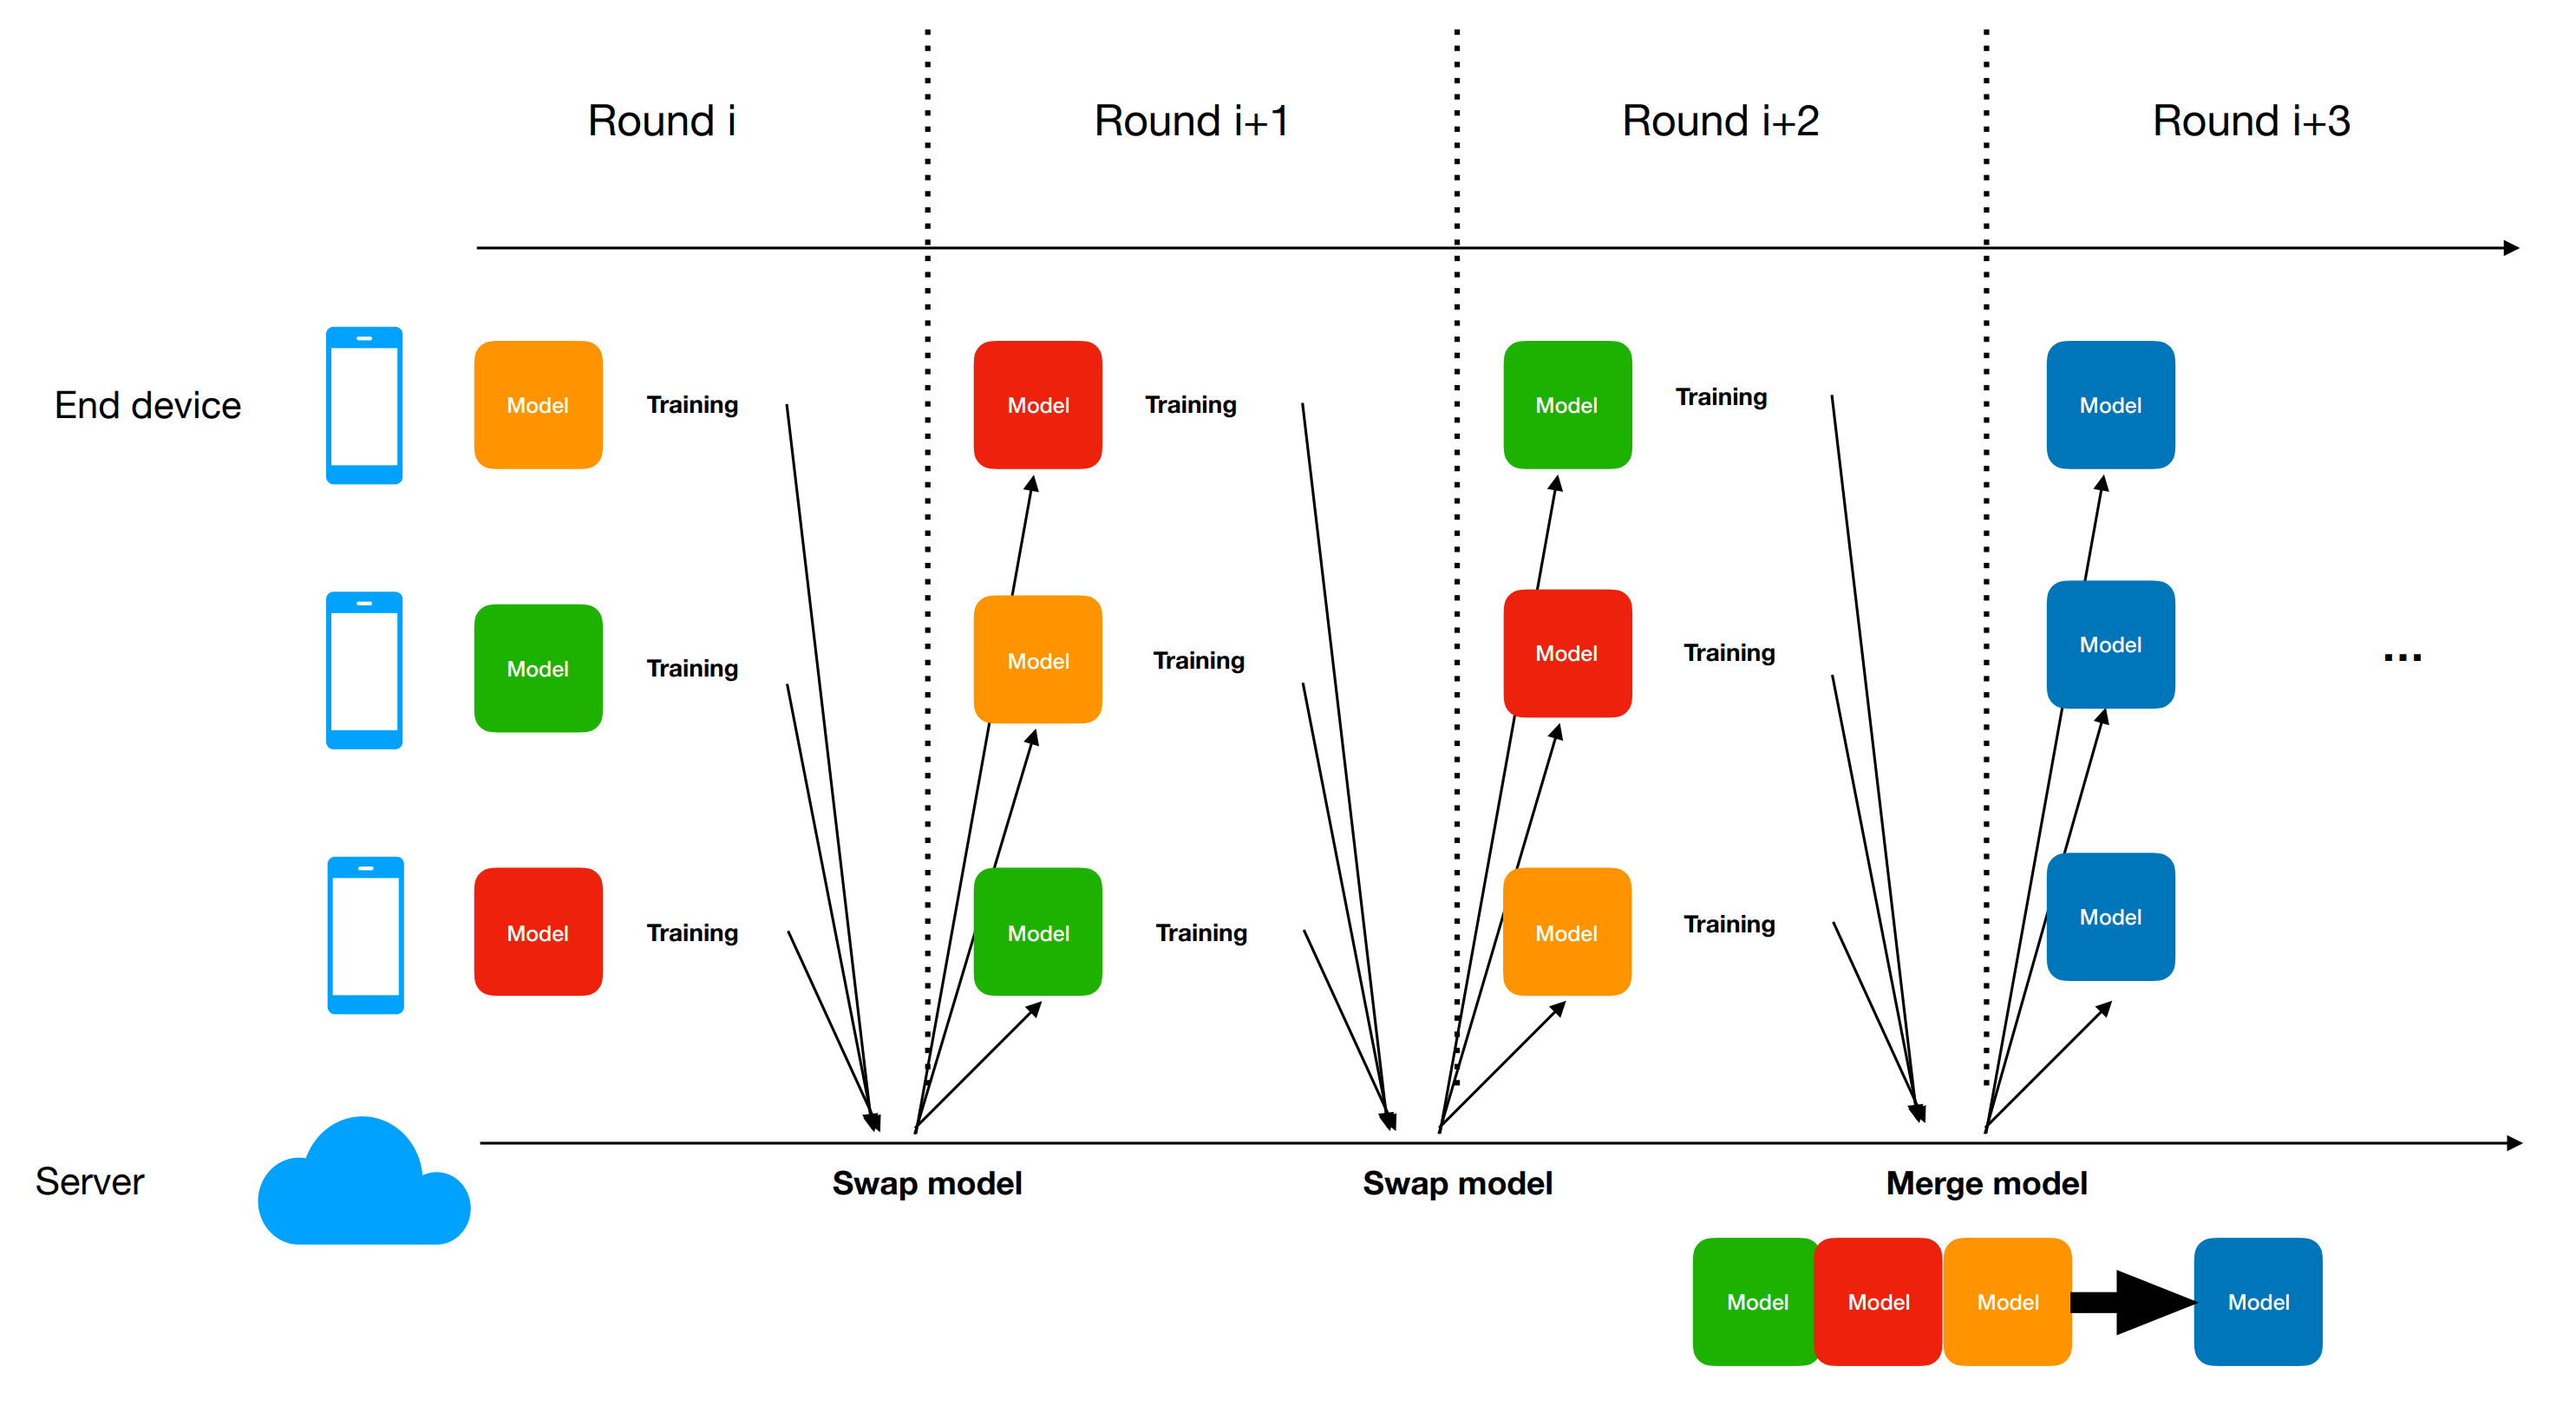
\includegraphics[scale=0.2]{images/chap4/federated_swapping.png}%
	\caption{%
		روش تعویض فدرال
		\cite{chiu2020semisupervised}%
		.
	}
	\label{federated_swapping}
	\centering
\end{figure}


برای حفظ عدالت در این فرآیند، از یک استراتژی چرخشی استفاده می‌شود. در این استراتژی، به طور منظم و به ترتیب، دو دستگاه نهایی به یکدیگر اجازه می‌دهند که مدل‌های خود را تبادل کنند. این کار باعث می‌شود که همه دستگاه‌های نهایی به طور مساوی در فرآیند تبادل مدل‌ها شرکت کنند و هیچ دستگاهی از مزایای این تبادل محروم نماند.

علاوه بر این، انتظار می‌رود که این عملیات تعویض مدل بین دستگاه‌های نهایی، به هر مدل دید گسترده‌تری از کل مجموعه داده‌ها بدهد. به عبارت دیگر، هر مدل محلی با تبادل مدل با دیگر دستگاه‌ها، می‌تواند اطلاعات بیشتری از داده‌های مختلف دریافت کند. این امر به کاهش انحراف وزن‌ها کمک می‌کند، زیرا مدل‌ها با داده‌های متنوع‌تری آموزش می‌بینند و به تدریج به یک مدل جامع‌تر و دقیق‌تر نزدیک می‌شوند.

به طور خلاصه، عملیات
\lr{FedSwap}
با تبادل مدل‌های محلی بین دستگاه‌های نهایی، نه تنها به بهبود دقت و عملکرد مدل‌ها کمک می‌کند، بلکه مشکلات ناشی از داده‌های
\lr{non-IID}
را نیز کاهش می‌دهد. این روش به عنوان یک رویکرد موثر در یادگیری فدرال می‌تواند باعث بهبود قابل توجهی در نتایج نهایی شود
\cite{chiu2020semisupervised}.


جزئیات عملیات
\lr{FedSwap}
در الگوریتم
\ref{algo_FedSwap}
ارائه شده است.
همچنین در جدول
\ref{tabel_FedSwapNotations}
نمادهای مختص این الگوریتم به نمایش در آمده است.
در این الگوریتم،
$w^k_t$
به عنوان وزن مدل در دستگاه نهایی
$k$
پس از گام
$t$
تنظیم می‌شود. در ابتدا، دستگاه‌های نهایی چندین به‌روزرسانی محلی انجام می‌دهند تا مدل‌های خود را بهبود بخشند. پس از هر
$h_1$
به‌روزرسانی محلی، سرور وارد عمل شده و عملیات
\lr{FedSwap}
را اجرا می‌کند. در این مرحله، مدل‌های محلی بین دستگاه‌های نهایی تبادل می‌شوند تا هر دستگاه بتواند از مدل‌های متنوع‌تری برای آموزش استفاده کند.

این تبادل مدل‌ها به کاهش تنوع داده‌ها بین دستگاه‌های مختلف کمک می‌کند و باعث می‌شود که مدل‌ها با داده‌های مختلفی آموزش ببینند. پس از انجام
$h_2$
عملیات
\lr{FedSwap}%
، سرور وارد عمل شده و عملیات
\lr{FedAvg}
را اجرا می‌کند. در این مرحله، سرور مدل‌های محلی را تجمیع می‌کند تا یک مدل مشترک ایجاد شود که از داده‌های تمام دستگاه‌ها بهره‌مند است.


\begin{LTR}
	\SetAlgoNlRelativeSize{-1}
	\begin{algorithm}[t]
		\begin{RTL}
			\caption{%
				تعویض فدرال
				\lr{(FedSwap)}
				\cite{chiu2020semisupervised}
			}
			\label{algo_FedSwap}
		\end{RTL}
		
		\begin{latin}
			Initialize all clients model with weight $w_0$\;
			\For{$t = 1, 2, \ldots, T$}{
				\For{each client $k = 1, 2, \ldots, K$
					\textbf{in parallel}}{
					$w_t^k = w_{t-1}^k - \eta \nabla F(w_{t-1}^k)$\;
				}
				\If{$t|h_1 = 0$ \quad and \quad $t|h_1h_2 \neq 0$}{
					\For{each client $k = 1, 2, \ldots, K$}{
						$w_t^k \gets \texttt{FedSwap}(k, \{w_t^k\}_{k \in K})$\;
					}
				}
				\If{$t|h_1h_2 = 0$}{
					$w_t \gets \texttt{FedAvg}(\{w_t^k\}_{k \in K})$\;
					\For{each client $k = 1, 2, \ldots, K$
						\textbf{in parallel}}{
						$w_t^k \gets w_t$\;
					}
				}
			}
			\SetKwFunction{FedSwap}{FedSwap}
			\SetKwFunction{FedAvg}{FedAvg}
			\SetKwProg{Fn}{Function}{:}{end}
			\Fn{\FedSwap{$k, \{w_t^k\}_{k \in K}$}}{
				$r$ \space represent a random client in \space $K$\;
				$w_t \gets w_t^r$\;
				$w_t^r \gets w_t^k$\;
				\KwRet $w_t$\;
			}
			\Fn{\FedAvg{$\{w_t^k\}_{k \in K}$}}{
				$w_t \gets \sum_{k=1}^K \frac{n_k}{n} w_t^k$\;
				\KwRet $w_t$\;
			}
		\end{latin}
	\end{algorithm}
\end{LTR}


\begin{table}[h]
	\centering
	\caption{نمادهای مختص الگوریتم
		\lr{FedSwap}
	}
	\label{tabel_FedSwapNotations}
	\begin{tabular}{cr}
		\hline
		متغیر & توضیحات \\
		\hline
		$h_1$ & تعداد گام‌ها بین هر
		\lr{FedSwap} \\
		$h_2$ & تعداد
		\lr{FedSwap}
		بین هر
		\lr{FedAvg} \\
		\hline
	\end{tabular}
\end{table}


برای تعیین مقادیر
$h_1$
و
$h_2$%
، ابتدا آزمایش‌های مختلفی انجام شده و بر اساس نتایج به دست آمده، بهینه‌ترین مقادیر انتخاب شده‌اند. در این آزمایش‌ها، چند نکته مهم مشاهده شده است. ابتدا، مقدار
$h_1$
به عملکرد به‌روزرسانی مدل محلی در دستگاه‌های نهایی وابسته است. از آنجایی که وظیفه یادگیری معمولاً یک وظیفه عمومی مثل طبقه‌بندی است، مقدار
$h_1$
بر اساس مقدار گام تعریف‌شده در روش میانگین‌گیری فدرال سنتی تنظیم می‌شود
\cite{chiu2020semisupervised}.

علاوه بر این، مقدار
$h_2$
نقش مهمی در توازن بین سربار ارتباطی و همگرایی مدل ایفا می‌کند. با افزایش مقدار
$h_2$%
، تعداد دفعات تعویض فدرال بین دستگاه‌های نهایی بیشتر خواهد شد. این امر می‌تواند با کاهش تعداد دفعات ادغام فدرال، پهنای باند ارتباطی بیشتری را صرفه‌جویی کند. با این حال، این امر ممکن است باعث افزایش احتمال انحراف وزن‌ها و کاهش دقت همگرایی مدل جهانی شود. به عبارت دیگر، هرچه مقدار
$h_2$
بزرگتر باشد، تعداد دفعاتی که مدل‌ها بین دستگاه‌های نهایی تعویض می‌شوند بیشتر است و این ممکن است به بهبود عملکرد مدل‌ها در مواجهه با داده‌های
\lr{non-IID}
کمک کند، اما ریسک انحراف وزن‌ها نیز بیشتر خواهد شد.

از سوی دیگر، اگر مقدار
$h_2$
کوچکتر باشد، فراوانی تعویض فدرال بین دستگاه‌های نهایی کاهش می‌یابد. این امر منجر به افزایش سربارهای ارتباطی می‌شود زیرا نیاز به ادغام مکرر مدل جهانی خواهد بود. بنابراین، مقدار
$h_2$
باید به گونه‌ای تنظیم شود که توازن مناسبی بین کاهش سربار ارتباطی و حفظ دقت مدل ایجاد کند.

در مجموع، روش
\lr{FedSwap}
با تعویض مدل‌های محلی بین دستگاه‌های نهایی بدون نیاز به هزینه‌های محاسباتی و ارتباطی اضافی، می‌تواند به بهبود عملکرد مدل‌ها در مواجهه با داده‌های
\lr{non-IID}
کمک کند
\cite{chiu2020semisupervised}.



\section{جابجایی مدل‌ها بر اساس میزان مشابهت}
در الگوریتم
\lr{FedSwap}%
، مدل‌ها بین دستگاه‌های نهایی جابجا می‌شوند. انتخاب دستگاه‌های نهایی جهت جابجایی به صورت کاملاً تصادفی انجام می‌گیرد، به این معنا که هنگامی که دو دستگاه می‌خواهند مدل‌های خود را جابجا کنند، فرآیند انتخاب این دو دستگاه به صورت کاملاً تصادفی انجام می‌شود. این تصادفی بودن انتخاب دستگاه‌ها باعث می‌شود که هیچ الگوی ثابتی در جابجایی مدل‌ها وجود نداشته باشد و هر بار ترکیب جدیدی از دستگاه‌ها در فرآیند تبادل مدل شرکت کنند.

یکی از ویژگی‌های مهم الگوریتم
\lr{FedSwap}
این است که تمام دستگاه‌های نهایی به صورت مساوی و عادلانه در این فرآیند جابجایی شرکت می‌کنند. به عبارت دیگر، همه دستگاه‌ها بدون استثنا در فرآیند جابجایی قرار می‌گیرند، اما انتخاب دستگاه‌ها برای جابجایی به صورت تصادفی صورت می‌پذیرد. این روش باعث می‌شود که تمامی دستگاه‌ها فرصت مساوی برای تبادل مدل‌ها و بهبود دقت و عملکرد خود داشته باشند.

با استفاده از این رویکرد، الگوریتم
\lr{FedSwap}
قادر است به بهبود عملکرد مدل‌های محلی کمک کند، زیرا تبادل تصادفی مدل‌ها بین دستگاه‌ها باعث می‌شود که هر دستگاه به داده‌ها و اطلاعات بیشتری دسترسی پیدا کند. این امر به کاهش انحراف وزن‌ها و بهبود همگرایی مدل جهانی کمک می‌کند.

%در الگوریتم FedSwap مدل‌ها بین دستگاه‌های نهایی جابجا می‌شوند ولی انتخاب دستگاه‌های نهایی جهت جابجایی به صورت کاملا تصادفی است یعنی هنگامی که دو دستگاه می‌خواهند مدل‌های خود را جابجا کنند این فرایند انتخاب دو دستگاه به صورت کاملا تصادفی صورت می‌پذیرد. در الگوریتم FedSwap تمام دستگاه‌های نهایی در این فرایند جابجایی به صورت مساوی و عادلانه شرکت خواهند کرد یعنی همه دستگاه‌ها بدون شک در فرایند جایجایی قرار خواهند گرفت ولی این انتخاب دستگاه نهایی برای جابجایی به صورت تصادفی صورت می‌پذیرد.



در این ‎پژوهش در نظر داریم که دستگاه‌های نهایی را بر اساس میزان شباهت‌ مدل‌‌های شبکه‌عصبی انتخاب کرده و در نهایت آن‌ها را با یکدیگر جابجا کنیم. پس در اینجا باید کامل با ساختار شبکه‌عصبی آشنا بوده و مدل‌ها شبکه‌عصبی را با یکدیگر مقایسه کنیم. همچینن باید در نظر داشت که بعد از بررسی مشابهت حال کدام مدل‌های موجود را با یکدیگر جابجا کنیم و اینجا بهترین انتخاب بدون شک مدلی است که کمترین شباهت را با مدل شبکه‌عصبی دستگاه فعلی دارد زیرا اگر مدل دستگاه فعلی با مدل دستگاه انتخابی مقصد شباهت زیادی داشته باشد این جابجایی اصلا مناسب نخواهد بود و مدل آموزش‌های لازم را نخواهد دید چون هنگامی که این شباهت بالا باشد بدین معناست که این دو دستگاه نهایی داده‌های یکسانی داشته و در طول این مدت مشابه یکدیگر آموزش دیده‌اند. 

پس در نتیجه در صورتی که مدل‌هایی با کمترین شباهت بین دستگاه‌های نهایی انتخاب شوند،‌ این فرض به این شکل مطرح می‌شود که با احتمال زیاد این دو دستگاه‌های داده‌هایی با ساختار متفاوت از یکدیگر داشته و این جابجایی مدل به صورت بهتری می‌تواند به فرایند یادگیری مدل کمک کرده و مدل را با داده‌های جدیدی روبه‌رو می‌کند و در نتیجه مدل سراسری زودتر به سمت مسیر بهینه همگرا خواهد شد.


کار بیشتر در سرور، مشکل محاسباتی وجود ندارد چون سرور مسئول این کار است و در یادگیری فدرال فقط فرض بر این است که دستگاه‌های نهایی دارای سخت‌افزاری قدرتمند نیستند و در اینجا نیز ما پردازش را بر روی دستگاه‌های نهایی نگذاشته‌ایم و این عملیات تنها بر روی سرور انجام می‌شود که آن هم از قدرت پردازش بالایی برخوردار است.


\section{معیار مشابهت}
تست

\subsection{CCA}
تست

\subsection{CKA}
تست

\subsection{نحوه پیداکردن مشابهت، لایه به لایه}
تست

\section{نحوه جستجوی کاربر نهایی جهت جابجایی مدل}
تست

\subsection{روش حریصانه}
تست

\subsection{روش بهینه}
تست





